\subsection{The Command Manager}

Queue management in Vulkan is a big and complex topic. Vulkan exposes the different queue families on your GPU, which support a subset of the following command types:

\begin{itemize}
    \item Graphics
    \item Transfer
    \item Compute
    \item Present
\end{itemize}

When submitting a command buffer to a queue, the queue needs to belong to a queue family, which supports the different types of the commands in the command buffer.

The management of Vulkan queues is completly up to the programmer. You can query the capabilities of the queue families and then enable an arbitrary amount of queues from different queue families. This is especially useful in a multi-threaded application, where you can submit two command buffers to two different queues and they will be executed in parallel.

The \code{CommandManager} class makes queue management easier. It manages the queue families, aswell as their enabled queues and created descriptor pools. Our application is signle-threaded in order to avoid too much complexity and because our main objective is to benchmark the performace of dynamic raytracing, which works better in a single-threaded environment. For this reason we also do not need multiple queues or queues designated for a certain type of operations (for example a designated transfer queue). However we do need a queue for every command type, which our command manager ensures. For every command type, it will iterate over all queue families and select the first family, which supports the command type. When creating the device, we enable the first queue of every queue family, which has been selected at least one time for a command type.

The following are some examples of possible queue setups:

\begin{figure}[H]
    \centering
    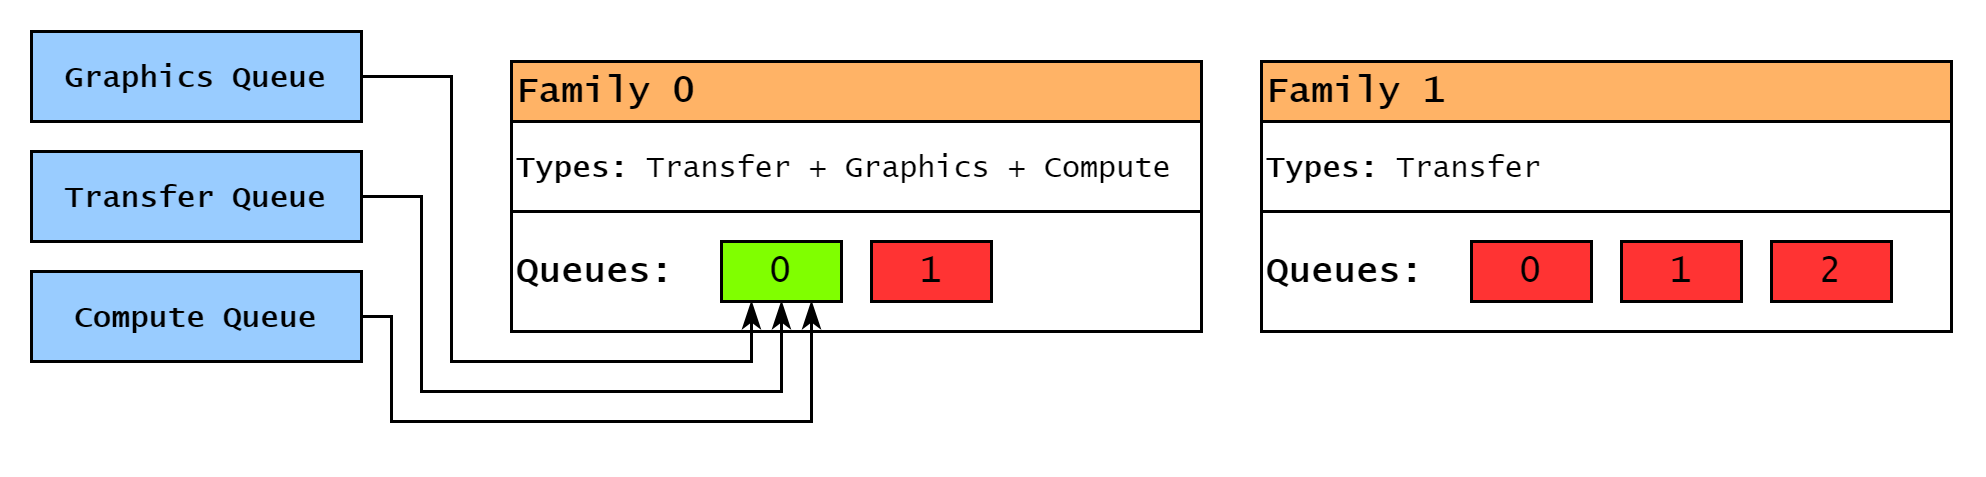
\includegraphics[width=1.0\textwidth]{figures/queue_setup_example_1.png}
    \caption{Queue setup example with only one queue}
    \label{fig:queue-example-1}
\end{figure}

\begin{figure}[H]
    \centering
    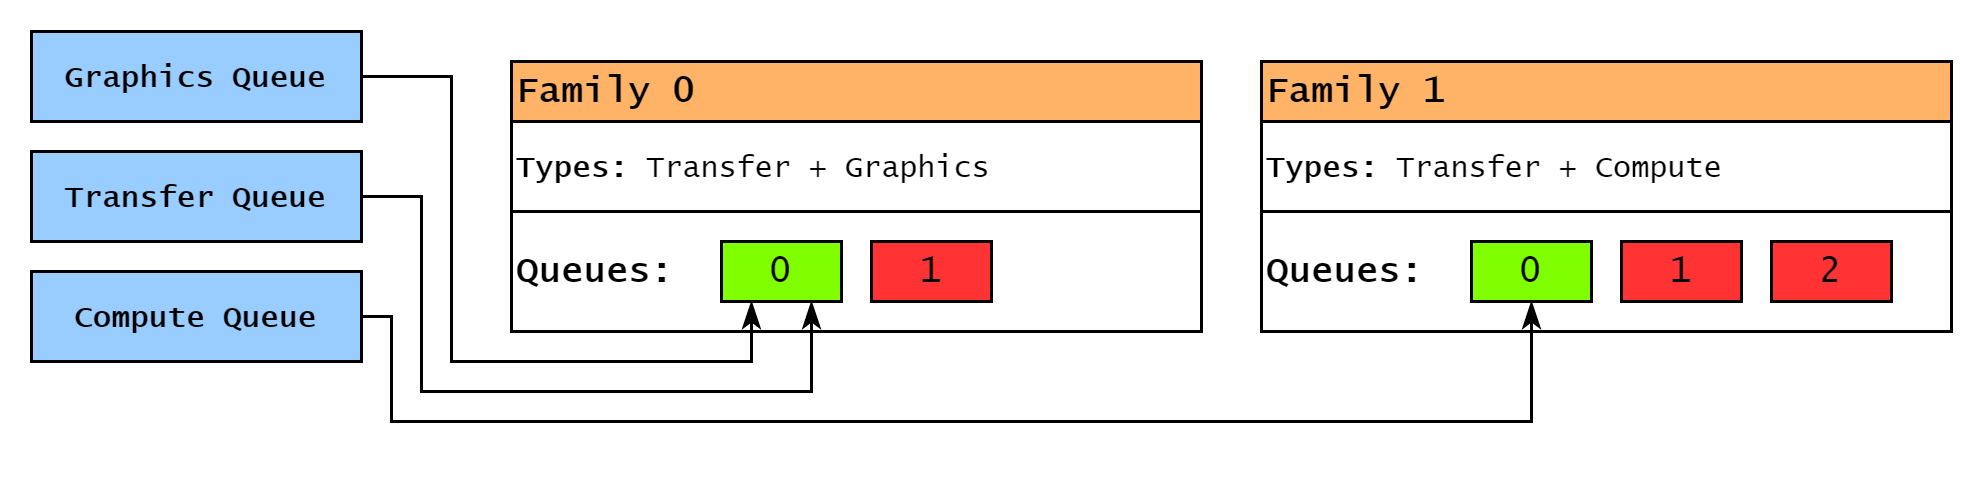
\includegraphics[width=1.0\textwidth]{figures/queue_setup_example_2.png}
    \caption{Queue setup example with two queues}
    \label{fig:queue-example-2}
\end{figure}

We also need a command pool to be able to allocate command buffers. When creating a command pool, a queue family has to be specified. Because the allocated command buffers can only be submitted to queues of the specified family, we create one command pool for every queue family that is used.

\subsection{The VMA Allocator}

As already mentioned in the chapter \nameref{chapter:technologies} (\autoref{subsec:vma}), our project uses VMA (Vulkan Memory Allocator) to make memory management in Vulkan easier. In order to be able to be allocate memory for our buffers and images later, we need an allocator. The allocator should be easily accessible when we create a buffer or image and for that reason we will also create and store the VMA allocator in the Vulkan context. We will use this allocator later, when allocation our resource objects (see \autoref{subsec:resource-objects}).

\subsection{Command Buffers}\label{subsec:command-buffers}

As we know, commands can not be executed in Vulkan directly, like they can for example in OpenGL. Instead, you first need to allocate a command buffer from a command pool. You can then record all of the commands you want to execute into the buffer and can then submit it for execution to a queue, that supports the type of the commands. It is important to note that when you submit the command buffer the current CPU-thread does not wait for all the commands to finish. This allows for the CPU to keep working, while the GPU runs our commands. If we want to wait for the command buffer to finish, we can specify a fence when submitting the command buffer, which will be signaled once all commands have finished.

We abstract this logic in the \code{CommandBuffer} class. It contains a \code{VkCommandBuffer} handle, a \code{Queue}, which tells the command buffer, where it should be submitted to, and a \code{Fence} (see \autoref{subsec:sync-objects}), which is used to wait for the command buffer to finish executing.

The \code{CommandBufferBuilder} has the following two parameters:

\begin{itemize}
    \item \textbf{\code{queue\_type}}: A value of type \code{QueueType}, which contains the elements \code{Transfer}, \code{Graphics}, \code{Compute} and \code{Present}. It is a mandatory parameter, which tells the builder to which of the queues inside the queue manager the command buffer is going to be submitted to (for example \code{QueueType::Graphics} means the command buffer will be submitted to the graphics queue of the command manager).
    \item \textbf{\code{single\_use}}: An optional boolean value, which is set to \code{false} by default. If set to \code{true}, it sets the \code{VK\_COMMAND\_BUFFER\_USAGE\_ONE\_TIME\_SUBMIT\_BIT} flag when recording the command buffer. This flag specifies, that the command buffer will only be submitted once, which lets the driver apply optimizations.
\end{itemize}

Inside \code{CommandBuffer} we can find the following member functions:

\begin{itemize}
    \item \textbf{\code{Ref record(CommandRecorder)}}:
    
    This function takes in a \code{CommandRecorder} as argument, which is an alias for \break \code{std::function<void(ReadyCommandBuffer)>}. In other words it is a function pointer or lambda function, which takes a \code{ReadyCommandBuffer} as an argument and returns \code{void}. A \code{ReadyCommandBuffer} is simply a wrapper around a \code{VkCommandBuffer} handle, which can only be constructed by the command buffer. The job of the \code{CommandRecorder} is, to record commands into the command buffer.

    Functions, that record a commands can be recognized by their \code{"cmd\_"} prefix. These functions have to be called inside a \code{CommandRecorder}, because thier first argument is always a \code{ReadyCommandBuffer}.

    \item \textbf{\code{Ref submit(SubmitInfo)}}:
    
    This function submits the command buffer to the queue, for which it was created for. The \code{SubmitInfo} parameter is optional and empty by default. This parameter allows us to specify semaphores, that we want to wait for before executing the command buffer, and semaphores, that we want to signal once the command buffer is finished executing (see \autoref{subsec:sync-objects}).

    \item \textbf{\code{Ref wait()}}:
    
    This functions simply waits for the execution of the command buffer to finish using a fence. If the command buffer is not currently getting executed, the function does nothing.

    It is also important to mention, that this function also gets called in the desctructor of the \code{CommandBuffer}, since it is not allowed to destroy a \code{VkCommandBuffer} while it is in execution. This also means, that a command buffer implicitly wait for execution to finish, when it goes out of scope.
    
    The underlying fence uses the flag \code{VK\_FENCE\_CREATE\_SIGNALED\_BIT}. Now if we call wait on a newly created command buffer, it will not block the thread, since the fence is signaled. We only reset the fence right before submitting the buffer for execution, because we only want to wait for the buffer while it is in execution.
\end{itemize}

The \code{CommandBuffer} class also contains the following static method:

\begin{center}
    \textbf{\code{static void single\_time\_submit(QueueType, CommandRecorder)}}
\end{center}

It creates a single-use command buffer for the queue with the specified \code{QueueType}. Then, it records the given \code{CommandRecorder}, submits it with an empty \code{SubmitInfo} and waits for execution to finish. It is basically just a quality-of-life function for creating and executing single-use command buffers.

The folloing code snippet shows, how the command buffer and its functions can be used:

\begin{figure}[H]
\centering
\begin{tabular}{c}
\begin{lstlisting}[language=C++]

// create the command buffer
CommandBuffer cmd_buf = CommandBufferBuilder()
    .queue_type(QueueType::Graphics)
    .single_use(true)
    .build();

// create a callback, which records the commands
CommandRecorder recorder = [&] (ReadyCommandBuffer ready_buf) {
    // record commands
    // ...
}

// record the commands, submit to queue and 
// wait for execution to finish in one line
cmd_buf.record(recorder).submit().wait();


\end{lstlisting}

\end{tabular}
\caption{An example of how to use command buffers in your code.}\label{fig:command-buffer}
\end{figure}

\subsection{Resource Objects}\label{subsec:resource-objects}
\textbf{Resource objects} are used to store data on the GPU, which can then be read and written to in shaders. In Vulkan we distinguish two types of resource objects:

\begin{itemize}
    \item \textbf{Buffer:}
    
    Buffers represent linear arrays of data which are used for various purposes by binding them to a graphics or compute pipeline via descriptor sets or certain commands, or by directly specifying them as parameters to certain commands~\parencite{vulkan-spec-resources}. The data is raw and not associated with any format, layout or dimensionality, therefore very flexible.

    Common usages:
    \begin{itemize}
        \item Vertex buffer
        \item Index buffer
        \item Uniform buffer
        \item Storage buffer
    \end{itemize}

    \item \textbf{Image:}

    Images are specialized resources that have multi-dimensional access rather than the typical linear access to memory~\parencite{vulkan-spec-images}. They can also be multi-dimensional and are associated with a format and layout.
    
    Common usages:
    \begin{itemize}
        \item Texture
        \item Render target
    \end{itemize}
\end{itemize}

We represent these two objects by the \code{Buffer} class and \code{Image} class. Since they are both resource objects, they are very similar in certain aspects. One challange, that they both share, is memory management, which can be quite difficult.

When creating a resource object, they are not actually backed by memory immediately, but you need to allocate a block of device memory and bind that memory to the resource. When allocating the memory, you need to specify a memory type, which corresponds to a certain memory heap and can have a set of properties, which impact the visibility of your memory aswell as performance. It is also important to mention, that too many allocations are not just bad for the performance of your application, but there is also a limit of allocations, that cannot be superceeded.

To make our lives a little bit easier, we use VMA (Vulkan Memory Allocator) (see \autoref{subsec:vma}).

The most important parameter we need, when using VMA is the \code{VmaMemoryUsage}, which describes the properties of the memory allocation. We use three of them in our project:

\begin{itemize}
    \item \code{\textbf{VMA\_MEMORY\_USAGE\_CPU\_ONLY}}:
    \item \code{\textbf{VMA\_MEMORY\_USAGE\_GPU\_ONLY}}:
    \item \code{\textbf{VMA\_MEMORY\_USAGE\_CPU\_TO\_GPU}}:
\end{itemize}

\subsection{Synchronization Objects}\label{subsec:sync-objects}

A lot of vulkan operations can be executed in parallel, which is why we need \textbf{synchronization objects}. There are two types:

\begin{itemize}
    \item \textbf{Semaphore:}
    
    A semaphore is used to synchronize two operations, which both happen on the GPU. We do this by specifying and array of wait-semaphores and an array of signal-semaphores. The GPU operation waits for all wait-semaphores to be signaled before starting and signals all signal-semaphores when it is finished.

    \item \textbf{Fence:}
    
    A fence is used to synchronize operations on the GPU with the CPU. This is done by specifying a fence when starting a GPU operation. When the GPU operation finishes, the fence gets signaled. The CPU can wait on a fence, which will block the thread until the fence gets signaled.
\end{itemize}

The \code{Semaphore} class encapsualtes a semaphore. It does not have any other functionality, other than holding a \code{VkSemaphore} handle (\autoref{subsec:basic-vulkan-object}), because it does not need it. A semaphore only ever gets passed as a parameter to GPU operations and these GPU operations signal and unsignal the semaphore. You never use the semaphore explicitly, but it is used implicitly by GPU operations. The \code{VkSemaphoreCreateInfo} does not have any member variables (other than \code{sType} and \code{pNext}). Therefore a builder would be a very clumsy way to create a semaphore. Instead we use the parameterless, static method \code{Semaphore::create}.

The \code{Fence} class encapsualtes a fence. While still being a very simple class, it does have a bit more functionality than \code{Semaphore}. A fence has two important member functions:

\begin{itemize}
    \item \code{\textbf{void reset()}}:
    
    This function resets the fences state to "unsignaled". A semaphore automatically gets set to unsignaled by the GPU operation that waits for it. Once a fence has been signaled, it will stay signaled until we manually reset it.

    \item \code{\textbf{void wait(uint64\_t timeout)}}:
    
    This function will block the current thread until the fence gets signeled or \code{timeout} nanoseconds pass. The \code{timeout} parameter is optional and set to \code{UINT64\_MAX}, which essencially makes the function indefinitly.
\end{itemize}

Eventhough \code{VkFenceCreateInfo} has one member variable, we use the static method \code{Fence::create} instead of a builder to create a fence. This method has the argument of type \code{VkFenceCreateFlags}. The \code{VkFenceCreateFlags} enum only contains the flag \code{VK\_FENCE\_CREATE\_SIGNALED\_BIT}. When setting this flag the fence will be created in the "signaled" state, otherwise the fence will be created in the "unsignaled" state. This is useful for our command buffer implementation (see \autoref{subsec:command-buffers}).

\subsection{Pipeline-related Objects}\label{subsec:pipeline-objects}

In this section we will talk about all the different Vulkan objects that are related to creating and using a pipeline. We will focus on the classical rasterization pipeline, which we also use for skinning in our application, but a lot of these objects are also used in the raytracing pipeline (see \autoref{subsec:raytracing-objects}).

\subsubsection{Shaders}

A \code{Shader} stores the code of a shader in Spir-V as well as the shader stage, that it is used in. The code can either be given directly in binary or be loaded from a specified file.

\subsubsection{Vertex Input}

The \code{VertexInput} struct describes the data, that gets passed to the vertex buffer. It has an array of \code{VertexBindingInfo}s and an array of \code{VertexAttributeInfo}s. Every binding info has a unique \code{binding} index, a \code{stride}, which is the distance between two elements in bytes, and an \code{input\_rate}, which specifies if an element should be read for every vertex or for every instance. Each attribute info is part of a specific \code{binding} (referenced by the binding index) and has a unique \code{location} index, an \code{offset} and a \code{format}. In order to access an attribute in the vertex shader, we need to specify its location (e.g. \code{layout(location = 0) in vec3 positions;}).

\subsubsection{Render Pass}

A \code{Renderpass} stores a set of \code{Attachment}s, that the shaders in a pipeline can output to. Each of these attachments holds information about their type (e.g. color, depth, stencil), format as well as load and store operations. Note that our implementation does not support stencil attachments, since they are never used in our project. Our appciation also does not allow sub-passes, or rather exactly one sub-pass per render pass.

\subsubsection{Framebuffer}

Just like an object is an instance of a class, a framebuffer can be seen as an instance of a render pass. It holds a set of image views, that are used as render targets. Each image views format and aspect needs to match their respective attachment in the render pass.

\subsubsection{Pipeline}

A pipeline describes the whole rendering process. It contains the render pass and the different shaders, vertex input and pipeline layout, as well as information for:

\begin{itemize}
    \item input topology
    \item rasterization
    \item depth testing
    \item color blending
    \item dynamic states
\end{itemize}

Most of this information is hard coded, since we dont need to change it in our application (depth testing, color blending, dynamic states). We can however change the input topology and disable rasterization (later used for GPU skinning).

\subsubsection{Pipeline layout and descriptor pool}

In order to be able to use data in a shader, that is not vertex data (e.g. uniform buffers, storage buffers, samplers, acceleration structures, ...), we need to describe the data using descriptor sets. These descriptor 

\subsection{Raytracing-related Objects}\label{subsec:raytracing-objects}